\chapter{Testing}

\section{Outline of Testing Strategy}
The majority of the focus with regards to testing for this project was on the platform's REST API. This is arguably the most important system within the platform and is where most (if not all) security issues are likely to happen. Therefore it was important that each feature is tested thoroughly.

In addition to the rigorous testing of the API, manual testing was completed for the Android and Web App. Although there are very capable automated testing libraries available for both Android and Angular (JUnit, Espresso, e2e, etc). Primarily, due to short-term time constraints, it was decided that manual tests would be the best approach. The acceptance criteria of each requirement were used as the testing criteria for a given story. 

Some informal user tests of the platform were also done towards the end of development. The primary focus of these tests was to ensure everything was in order and functioning properly for the final demonstration. However, they served perfectly to compliment the testing strategy already in place. 

\section{Testing the API}
All of the API's testing was done on a 'per-route' basis, meaning, after successful implementation was completed, automated tests were written to rigorously test each route. This approach was selected because each of the platform's features was being implemented via a route within the REST API. Therefore it made sense to thoroughly test each route and by extension, each feature. There are roughly 5-6 tests for each route, making a total of 85 automated tests. 

\subsection{Testing Technologies Used}
In order to create the automated tests a few third party libraries were used: Mochajs, Chaijs, and Mockgoose. Mochajs was used to create a testing environment for NPM to run (within a Docker container). Chaijs is an assertion library with support for HTTP requests. Therefore within each test block, a Chai HTTP request was sent to the API and the response was evaluated using Chai's 'should' library.

Mockgoose is an NPM package that provides a test environment-friendly database by spinning up an in-memory MongoDB database. It 'catches' any requests made through Mongoose and forces them to be executed on the in-memory database as opposed to the standard data volume. By using an in-memory database tests can be run within the environment with zero consequence for the actual persisted data, whilst still maintaining the reliability of using a production DBMS.

\subsection{Regression Testing}
By using  TravisCI, the continuous integration tool all tests are automatically executed whenever the API is pushed to GitHub. If a test fails an email notification is sent out and the build is marked as 'failed'. This was invaluable during development to force regression tests to be executed whenever a new feature was pushed to the repository. Thus reducing the risk of bugs and hopefully increasing the correctness of the software.

\subsection{Stress Testing}
A major advantage of the chosen testing strategy is that automated tests can be used to accurately perform stress tests on the platform. For each route, a number of edge cases and fail conditions are tested. For example, for any route with input validation, attempted submission with invalid or incorrect input is simulated. The correct response to such a simulation is then asserted.

\subsection{Security Testing}
In addition to the stress testing undertaken, aspects of the API's security are also tested. For security testing, a mixture of automated tests and manual testing using Postman~\cite{postman_documentation_ref} were used. For example, most protected routes have automated tests to enforce the correct behaviour if invalid tokens are provided. The 'GET /users/{id}' route has an automated test to ensure that if a user's record is successfully retrieved their hashed password is not included in the response.

\section{Manually Testing the User-Facing Applications}
In order to test the user-facing applications within the platform as comprehensively as possible given the time restrictions, a manual approach was adopted. With acceptance criteria already being in place for each user story, the pass criteria of the manual tests were effectively already in place. 

Admittedly, much of the UI testing for the Android App was impromptu attempts at breaking or crashing the Android App. This was especially true with the Android App's handling of screen orientation. However, much of the UI testing also had a methodical approach. For example, when a new feature was fully implemented, a run-through of the process was done using Postman as the API's client. Then again using the Android App, then the results were compared to ensure correctness.

With regards to the Web Application's UI testing, many of the interface's elements were provided by reliable third-party code and were therefore inherently robust. However, some manual testing was done on the aspects of the interface implemented solely for the platform. The Web Application was also consistently tested for its support on various device resolutions.

\section{User Testing of the Platform}
As discussed at the beginning of the section, the platform in its entirety underwent informal user testing. Acquaintances had volunteered to simulate a potential use-case of the platform. One person would play the role of a customer using a mobile device, another would play the role of a driver, and a third would use a desktop device and play the role of a Company Admin. In order to fully commit to the simulation and hopefully give an idea of the platform's performance in a real-world scenario, the person playing the role of the driver used the Android App from a phone mount within a parked car.

The user testing was mainly focused on gauging the usability of the platform as a whole and preparing for the final demonstration. It was not intended to be a primary aspect of the testing strategy. However, having loaded the App onto one of the participant's devices (Samsung Galaxy S9 Running Android Pie), it was discovered that the App was throwing a network error. Because the App is consuming the API via HTTP, devices running a more up-to-date version of Android were rejecting the calls. The fix was simple and involved the simple addition of a line in the AndroidManifest file. However, if the test had not been completed, this issue would likely have occurred in the project's final demonstration.

\begin{figure}[!h]
	\centering
	\begin{subfigure}[b]{0.6\linewidth}
		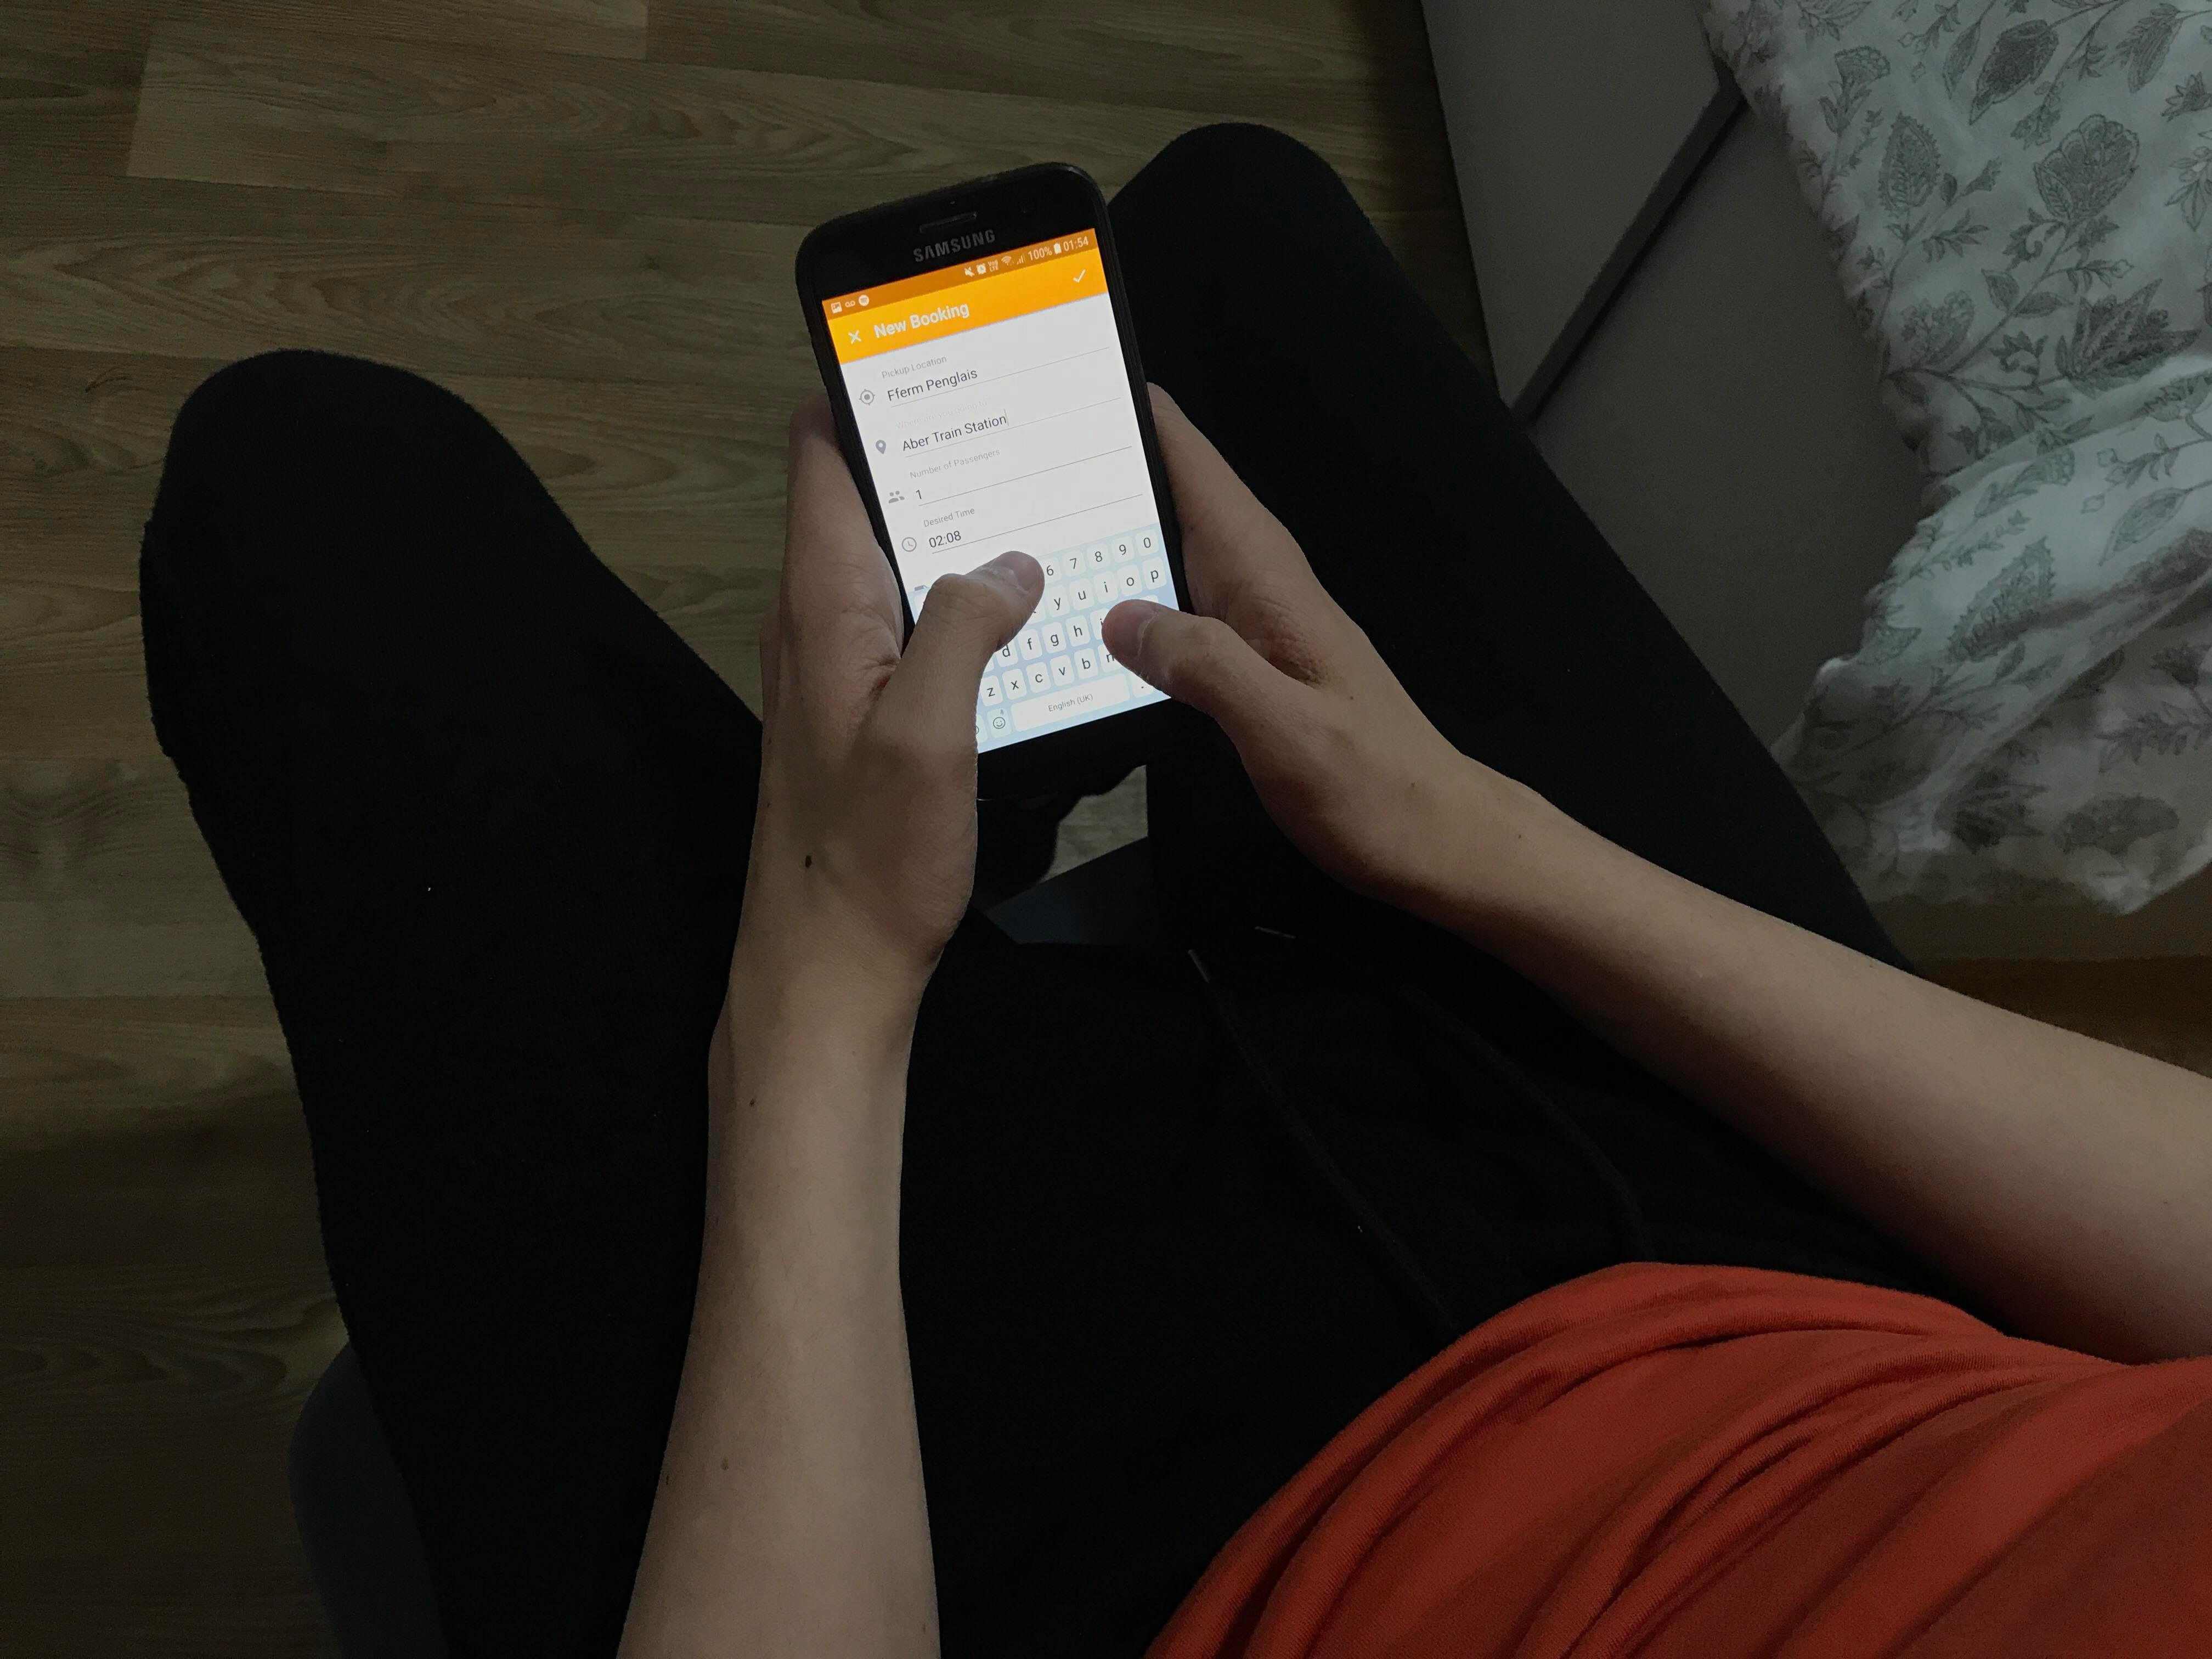
\includegraphics[width=\linewidth]{Resources/img/user_test_customer.jpg}
		\caption{Customer}
	\end{subfigure}
	\begin{subfigure}[b]{0.6\linewidth}
		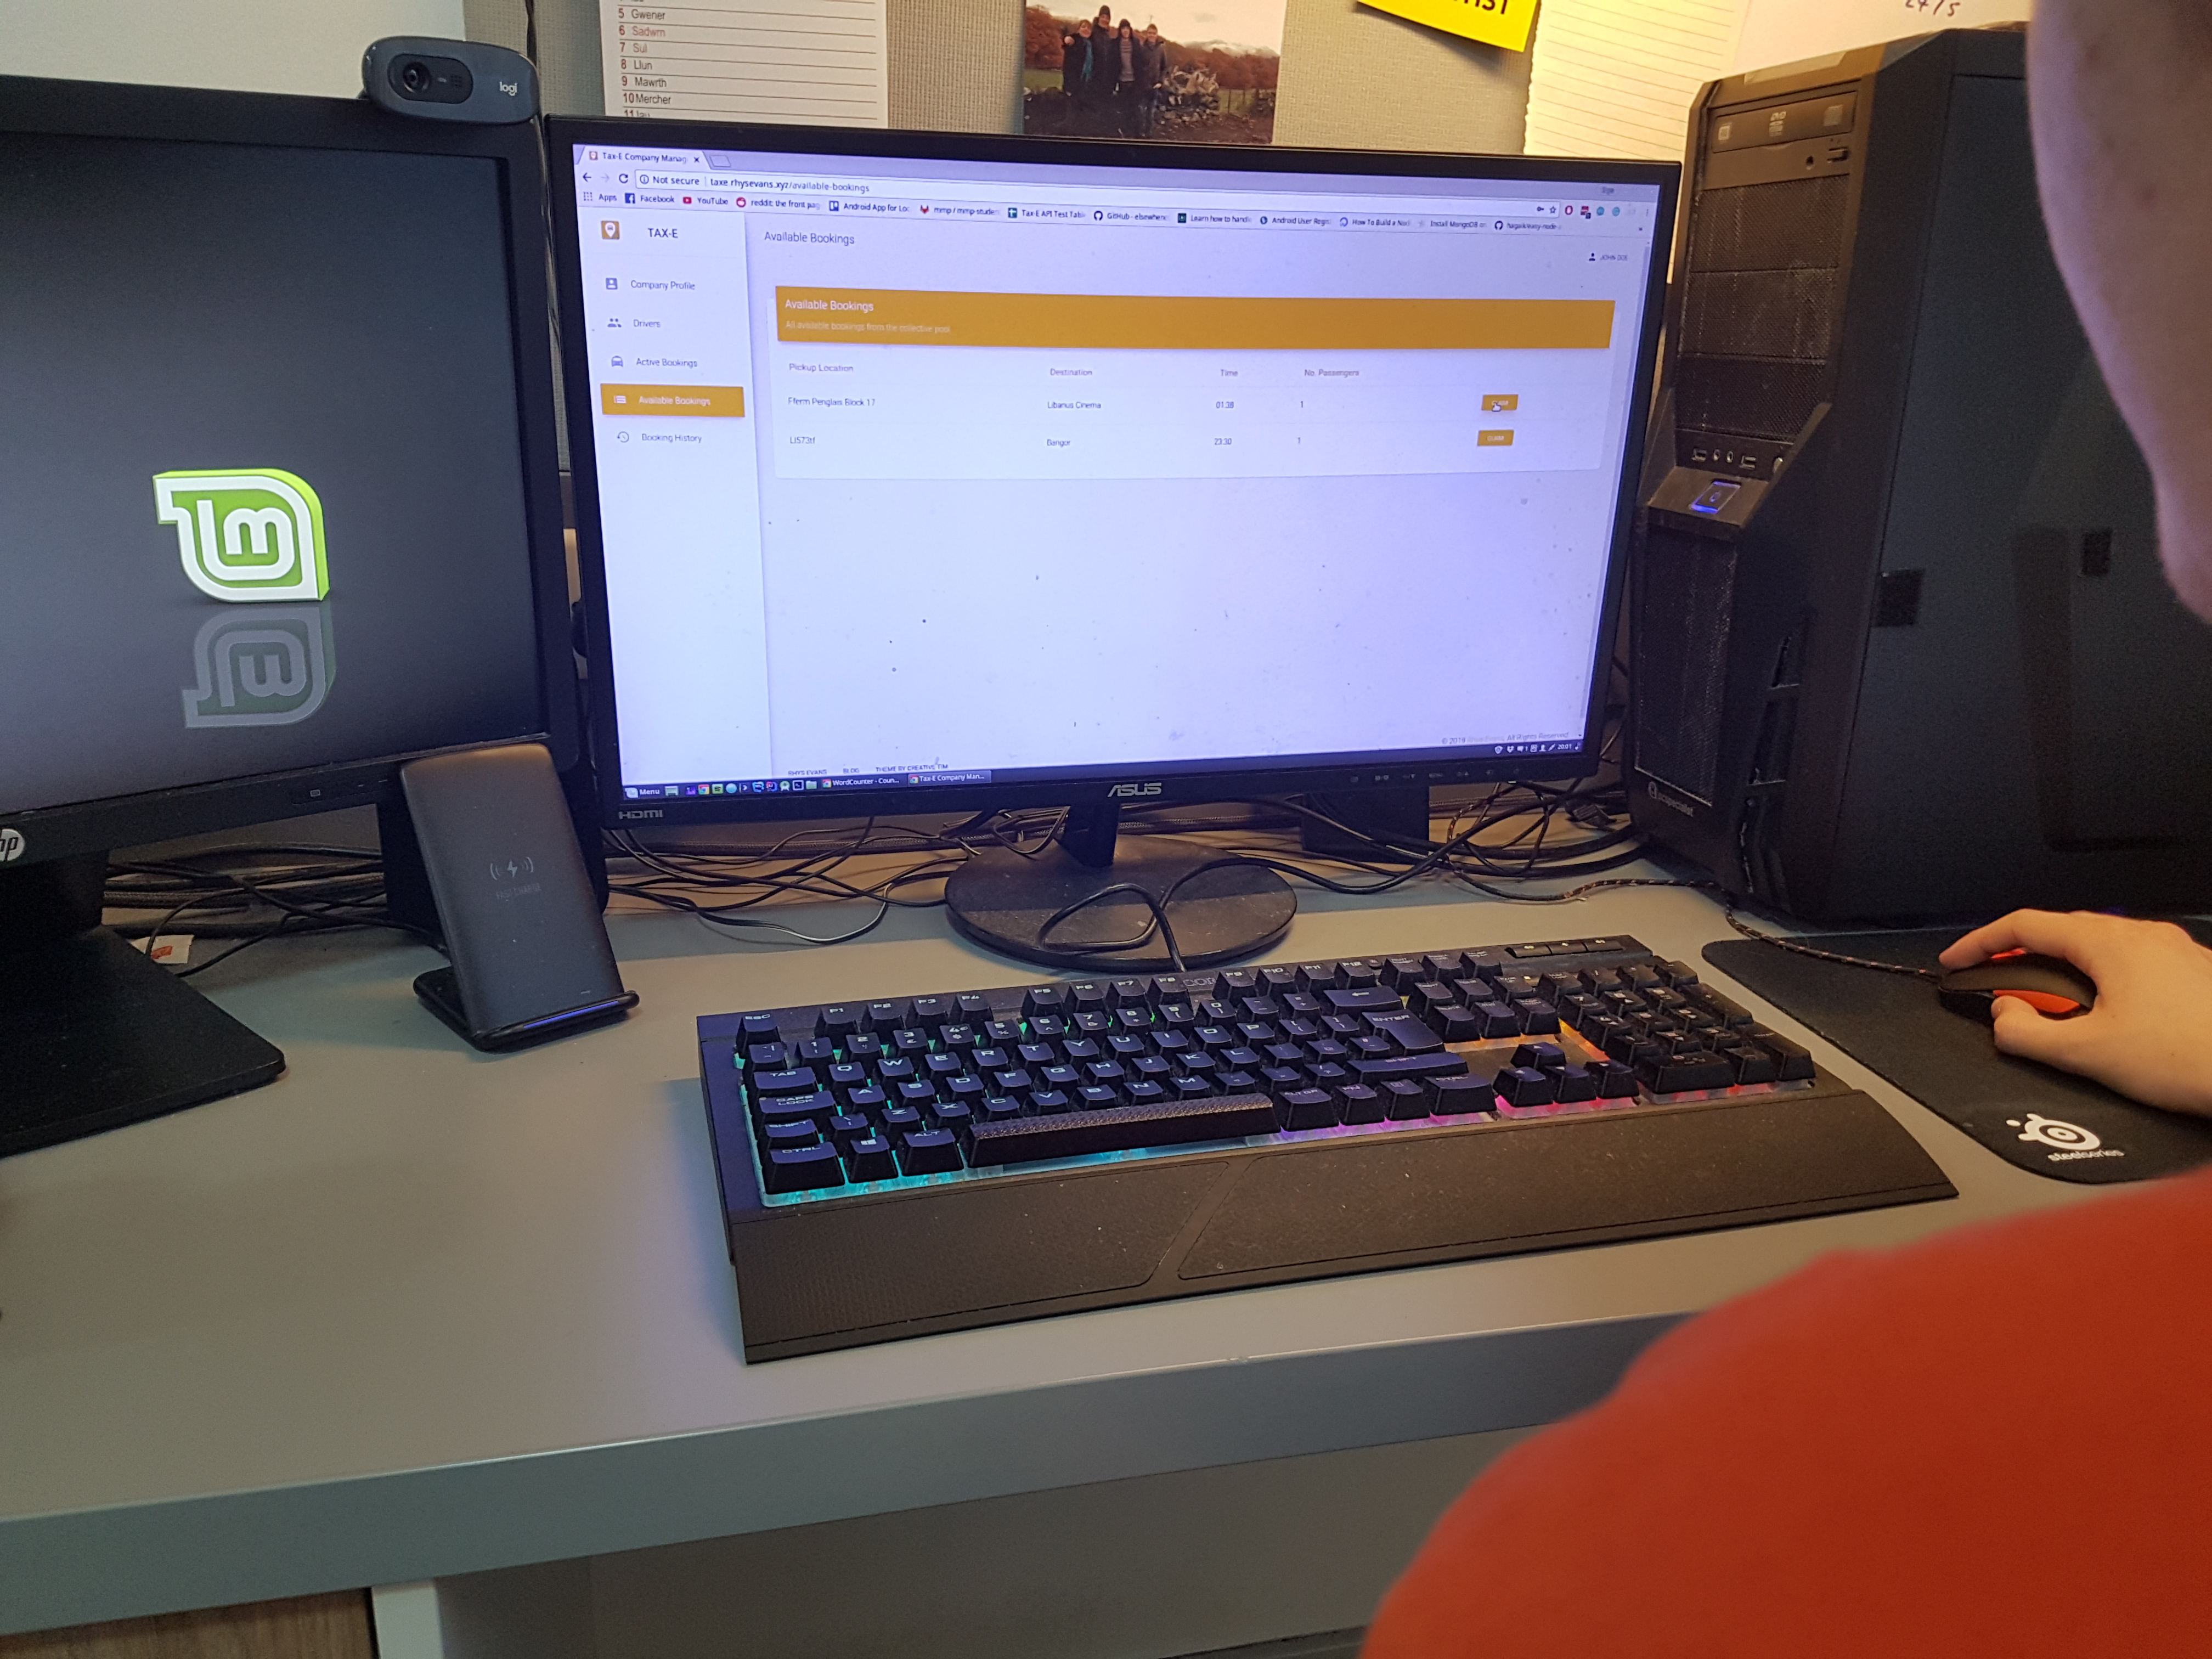
\includegraphics[width=\linewidth]{Resources/img/user_test_admin.jpg}
		\caption{Company Admin}
	\end{subfigure}
	\begin{subfigure}[b]{0.6\linewidth}
		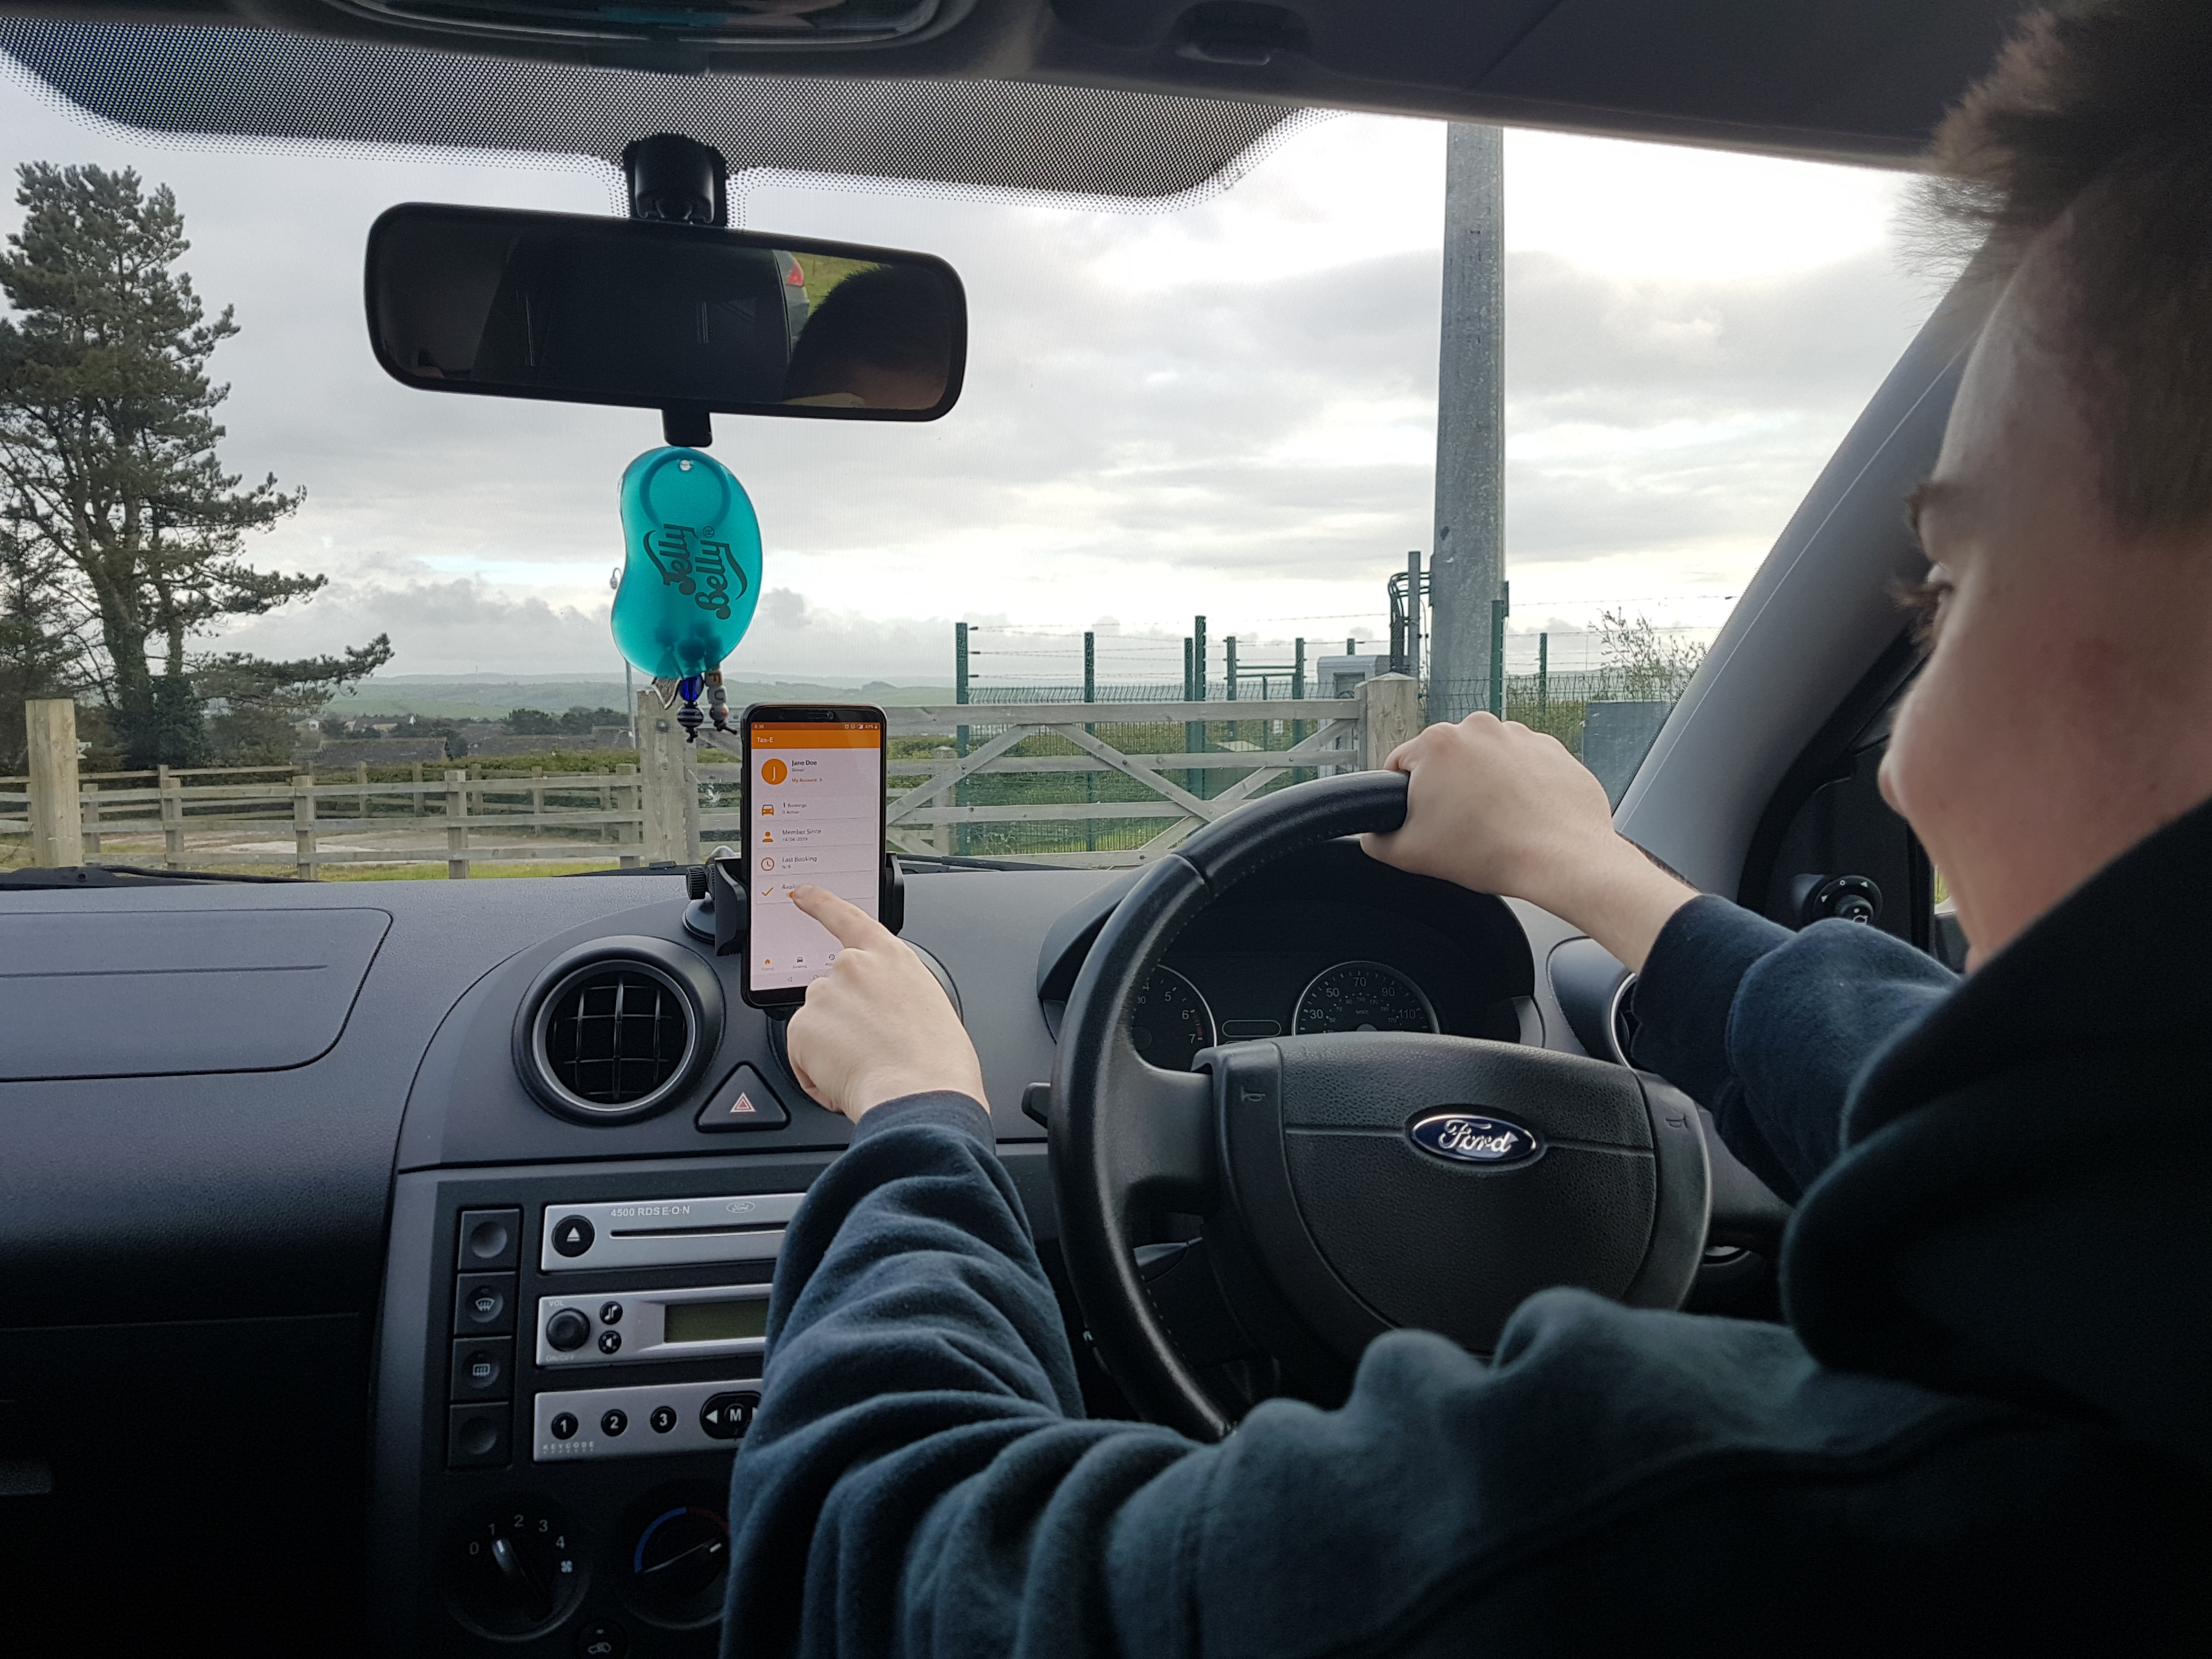
\includegraphics[width=\linewidth]{Resources/img/user_test_driver.jpg}
		\caption{Driver}
	\end{subfigure}
	\caption{Photographs of the User Testing Process}
	\label{fig:user_testing}
\end{figure}